 \documentclass{beamer}

\usetheme{MagdeburgFIN}
\usefonttheme{structurebold}
\usepackage{graphicx}
\usepackage{float}
\usepackage{url}
\usepackage{pdfpages}
\usepackage{mathtools}
\usepackage{algorithm}
\usepackage{caption}


\title{Computational Intelligence in Games}
\author{Emergence}
\date{\today}
\institute{Otto-von-Guericke-University Magdeburg}


\begin{document}


\begin{frame}[plain]
 \titlepage
\end{frame}

% Fred
\begin{frame}
\frametitle{Agenda}
\begin{itemize}
\item Dummy
\item Dummy
\item Dummy
\item Dummy
\item Dummy
\end{itemize}
\end{frame}


% Julian
\begin{frame}
\frametitle{Heuristic Agent I}
\begin{itemize}
\item Dummy
\end{itemize}
\end{frame}

\begin{frame}
\frametitle{Heuristic Agent II}
\begin{itemize} \item Dummy
\end{itemize}
\end{frame}


\begin{frame}
\frametitle{Heuristic Agent III}
\begin{itemize}
 \item Dummy
\end{itemize}
\end{frame}

\begin{frame}
\frametitle{Heuristic Agent IV}
\begin{itemize}
 \item Dummy
\end{itemize}
\end{frame}



% Fred
\begin{frame}
\frametitle{MCTS}
\begin{itemize}
 \item Dummy
\end{itemize}
\end{frame}

\begin{frame}
\frametitle{MCTS Agent I}
\begin{itemize}
 \item Dummy
\end{itemize}
\end{frame}

\begin{frame}
\frametitle{MCTS Agent II}
\begin{itemize}
 \item Dummy
\end{itemize}
\end{frame}


% Julian
\begin{frame}
\frametitle{EA}


\end{frame}





\begin{frame}
\frametitle{EA Agent I}

DeltaScoreEvaluation function 
\begin{equation*}
s = \sum_{t=0}^n (H(s_t) - H(s_{t-1}))
\end{equation*}

is calculated by using the function

\begin{equation*}
    H(s_i, s_{i-1}) = 
\begin{dcases}
    10, & \text{if isWinner}  \\
    -10, & \text{if isLooser}  \\
    score(s_i) - score(s_{i-1}), & \text{otherwise.}
\end{dcases}
\end{equation*}
\end{frame}



\begin{frame}
\frametitle{EA Agent II}
\begin{figure}[H]
\centering
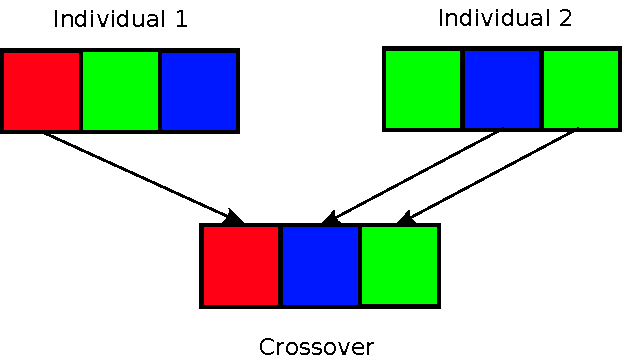
\includegraphics[scale=0.6]{../report/images/crossover.pdf}
\caption{Crossover of an individual}
\label{fig:crossover}
\end{figure}
\end{frame}


\begin{frame}
\frametitle{EA Agent III}
\begin{figure}[H]
\centering
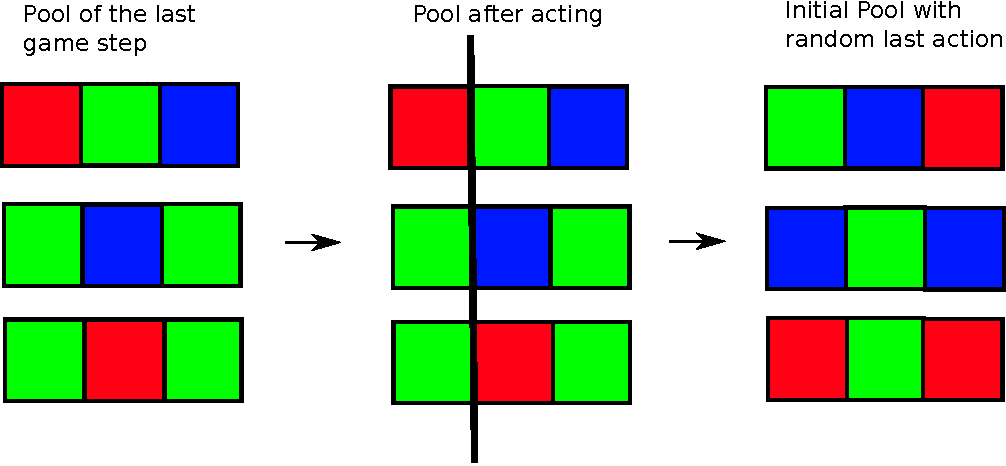
\includegraphics[scale=0.6]{../report/images/sliding_window.pdf}
\caption{Sliding Window}
\label{fig:sliding_window}
\end{figure}
\end{frame}


% Julian
\begin{frame}
\frametitle{Experiment Result I}
\begin{itemize}
 \item Dummy
\end{itemize}
\end{frame}

\begin{frame}
\frametitle{Experiment Result II}
\begin{itemize}
 \item Dummy
\end{itemize}
\end{frame}


\begin{frame}
\frametitle{Experiment Result III}
\begin{itemize}
 \item Dummy
\end{itemize}
\end{frame}



% Fred
\begin{frame}
\frametitle{Development Process}
\begin{itemize}
 \item Dummy
\end{itemize}
\end{frame}


\begin{frame}
\frametitle{Main Problems Difficulties}
\begin{itemize}
 \item Dummy
\end{itemize}
\end{frame}


\begin{frame}
\frametitle{Conclusion \& Future Work}
\begin{itemize}
 \item Dummy
\end{itemize}
\end{frame}




\begin{frame}
\begin{center}
\frametitle{Thank you for your attention!}
\end{center}
\end{frame}


\end{document}
